% 2018 江苏卷第18题：椭圆与焦点直径圆
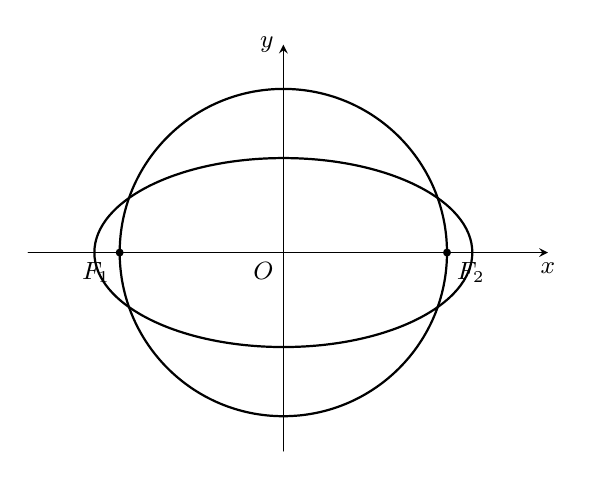
\begin{tikzpicture}[font=\small, line cap=round, line join=round, >=stealth, scale=1.2]
  % 坐标轴
  \draw[->] (-2.7, 0) -- (2.8, 0) node[below] {$x$};
  \draw[->] (0, -2.1) -- (0, 2.2) node[left] {$y$};
  \node[below left] at (0, 0) {$O$};

  % 椭圆: x^2/4 + y^2 = 1 (a=2, b=1)
  \draw[thick] (0, 0) ellipse (2cm and 1cm);

  % 圆: x^2 + y^2 = 3 (r = sqrt(3) ≈ 1.732)
  \draw[thick] (0, 0) circle (1.732cm);

  % 焦点 F1(-sqrt(3), 0), F2(sqrt(3), 0)
  \coordinate (F1) at (-1.732, 0);
  \coordinate (F2) at (1.732, 0);
  \fill (F1) circle (1.2pt) node[below left] {$F_1$};
  \fill (F2) circle (1.2pt) node[below right] {$F_2$};
\end{tikzpicture}
